\documentclass{beamer}

\usepackage{fontspec}
\usepackage{amsmath}
\usepackage{hyperref}
\usepackage[backend=biber]{biblatex}
\usepackage{tikz}
\usepackage{expl3}
% \usepackage{euler-math}
\usepackage[export]{adjustbox}
\usepackage{bm}
\usepackage{neuralnetwork}
\usepackage{graphicx}
\usepackage{minted}

\usetikzlibrary{quantikz}
\usetikzlibrary{fadings}

\ExplSyntaxOn
\newcommand{\braopket}[3]{\langle #1 | #2 | #3 \rangle}
\newcommand{\expected}[1]{\langle #1 \rangle}
\DeclareMathOperator{\Tr}{Tr}
\DeclarePairedDelimiter\abs{\lvert}{\rvert}
\DeclarePairedDelimiter\norm{\lVert}{\rVert}
%% quantikz provides \Pr \proj \bra \ket \braket
\ExplSyntaxOff


\usefonttheme{professionalfonts}
\setmainfont{TeX Gyre Pagella}
\setsansfont{TeX Gyre Heros}
\setmonofont{IBM Plex Mono}

\newfontfamily\headingfont{TeX Gyre Heros Bold}
\setbeamerfont{title}{family=\headingfont}
\setbeamerfont{frametitle}{family=\headingfont}
\setbeamerfont{math text}{series=\fontseries{AMS Euler}}

\setbeamertemplate{title page}[default][left]
\setbeamercolor{frametitle}{fg=black}
\setbeamertemplate{items}[circle]
\setbeamercolor{item}{fg=black}

\setbeamertemplate{headline}[default]

\setbeamertemplate{navigation symbols}{}
\useoutertheme{miniframes}
\setbeamercolor*{mini frame}{fg=black}

\addbibresource{cpen400q.bib}

\title{Experimental Quantum GANs}
\subtitle{CPEN 400Q class presentation}
\author{Yuyou Lai, Juntong Luo, Sam Schweigel, Bolong Tan}
\date{}
\titlegraphic{
    \begin{tikzpicture}
        \node (img0) at (0,0) {\includegraphics[width=0.6\linewidth,clip,trim=130 677 285 90,page=3]{figures/original-paper.pdf}};
        \node (img1) at (0,-1) {\includegraphics[width=0.6\linewidth,clip,trim=353 677 63.2 90,page=3]{figures/original-paper.pdf}};
    \end{tikzpicture}
}

\begin{document}

% Disable the header/footer
\setbeamertemplate{headline}{}
\setbeamertemplate{footline}{}
\frame{\titlepage}

% Enable the contents header
\makeatletter
\setbeamertemplate{headline}{%
  \vspace{1em}%
  \insertnavigation{\paperwidth}%
  \vspace{1em}%
}%
% \setbeamertemplate{footline}{%
%   \usebeamerfont{footline}%
%   \usebeamercolor[fg]{footline}%
%   \hfill%
%   \insertframenumber\hspace{1em}%
%   \vspace{1em}%
% }%
\makeatother

\section{Overview}
% \begin{frame}
%   We implemented some of the ideas from \emph{Experimental Quantum Generative
%   Adversarial Networks for Image Generation}\autocite{huang2021} by Huang et al.

%   \begin{center}
%     \vfill
%     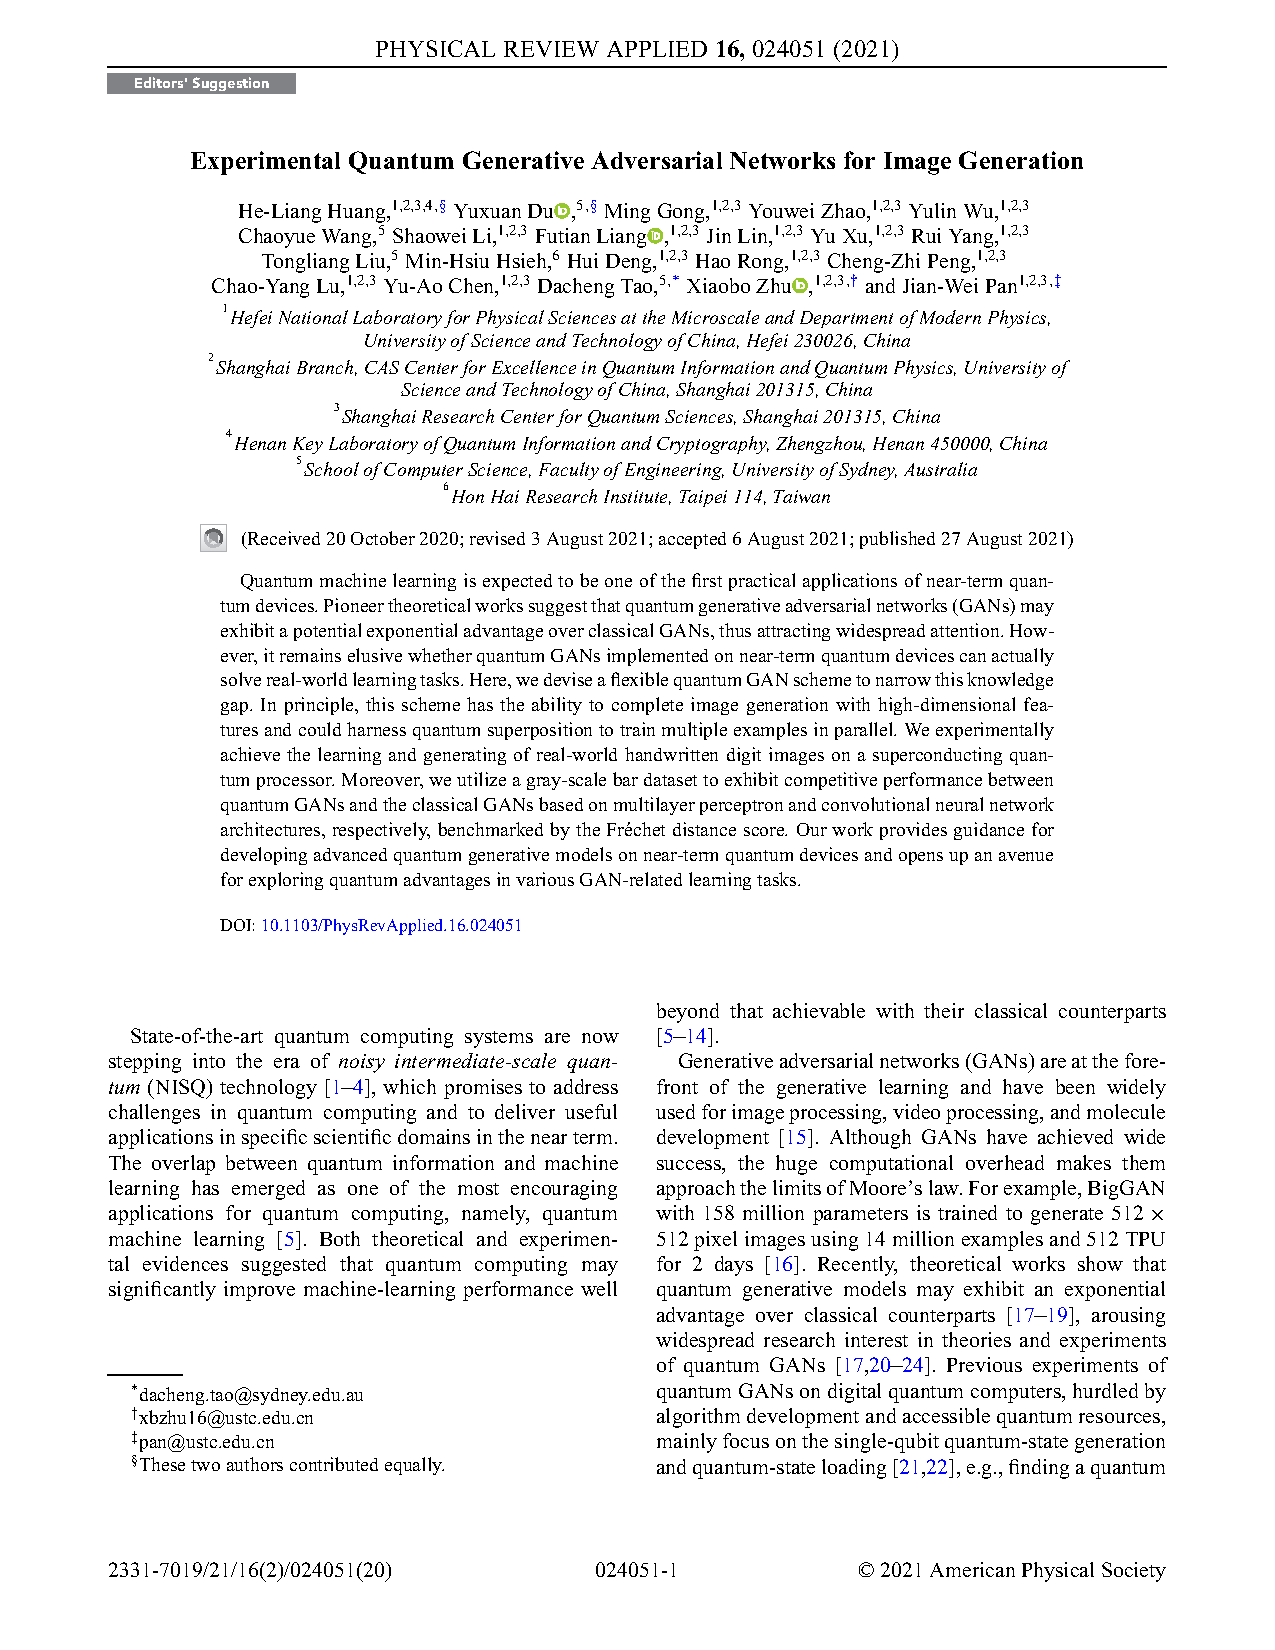
\includegraphics[width=0.8\linewidth,clip,frame,trim=0 500 0 0,page=1]{figures/original-paper.pdf}%
%     \\[-4em]%
%     \begin{tikzpicture}
%       \fill[white,path fading=north] (0,-3em) rectangle (0.81\linewidth,0);
%       \fill[white] (0,-3em) rectangle (0.81\linewidth,-4em);
%     \end{tikzpicture}% lol
%   \end{center}
% \end{frame}

% Terence
% - key findings and results of paper

\begin{frame}{Overview}
\begin{itemize}
    \item "Experimental Quantum Generative Adversarial Networks for Image Generation"
    \item Implemented quantum GANs on a real quantum device. 
    
    \item They achieve the learning and generating of real-world 
    \hspace{0.4cm} handwritten 2X2 digit images on a superconducting \hspace{0.4cm} quantum processor.

\item Two training strategies: 

    Batch: Training the GAN on batches of images
    
    Patch: Dividing the image into smaller patches and training 
    
    \hspace{1.1cm} the GAN on each patch individually
    
\end{itemize}
\end{frame}


\section{Background}
% Robin

\begin{frame}
\frametitle{Neural Networks}
\begin{itemize}
\item Neural networks are a type of machine-learning model inspired by the structure of the human brain.
\begin{figure}[h]
\centering
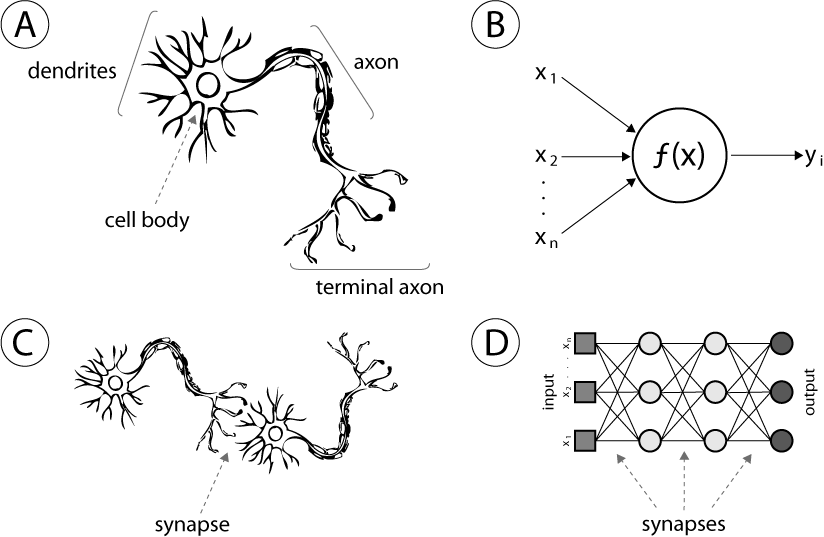
\includegraphics[width=0.7\textwidth]{figures/neural_brain.png}
% \caption{My image with a reference \cite{https://wp.nyu.edu/yungjurick/2020/03/15/debate-on-the-relationship-between-neural-network-and-the-brain/}}
% \label{fig:my_image}
\end{figure}
\item neural network can learn to recognize patterns and make predictions based on input data, it can be used for image and speech recognition, natural language processing, etc.

\end{itemize}
\end{frame}

% \begin{frame}
% \frametitle{Neural Networks}
%     % \begin{neuralnetwork}[height=4]
%     %     \newcommand{\x}[2]{$x_#2$}
%     %     \newcommand{\y}[2]{$\hat{y}_#2$}
%     %     \newcommand{\hfirst}[2]{\small $h^{(1)}_#2$}
%     %     \newcommand{\hsecond}[2]{\small $h^{(2)}_#2$}
%     %     \inputlayer[count=3, bias=true, title=Input\\layer, text=\x]
%     %     \hiddenlayer[count=4, bias=false, title=Hidden\\layer 1, text=\hfirst] \linklayers
%     %     \hiddenlayer[count=3, bias=false, title=Hidden\\layer 2, text=\hsecond] \linklayers
%     %     \outputlayer[count=2, title=Output\\layer, text=\y] \linklayers
%     % \end{neuralnetwork}
% \begin{itemize}
% \end{itemize}
% \end{frame}

\begin{frame}
\frametitle{Generative Adversarial Network (GAN)}
\begin{itemize}
\item GAN is a specific type of neural network that are used for generating new data that is similar to a given dataset.
\begin{figure}[h]
\centering
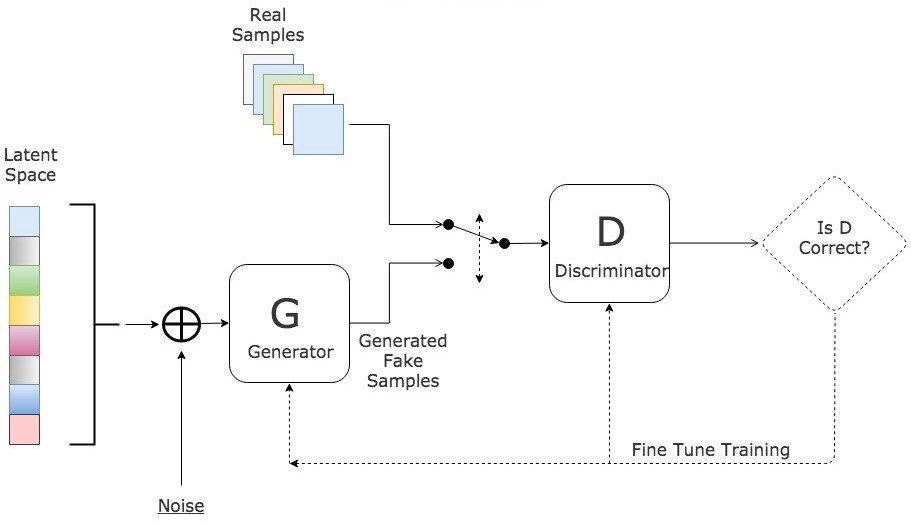
\includegraphics[width=0.8\textwidth]{figures/gan.jpeg}
% \caption{My image with a reference \cite{https://wp.nyu.edu/yungjurick/2020/03/15/debate-on-the-relationship-between-neural-network-and-the-brain/}}
% \label{fig:my_image}
\end{figure}
\item GANs consist of two neural networks: a generator and a discriminator.
\end{itemize}
\end{frame}


\section{Theory}
% Sam
% - maybe MPQCs?

% \begin{frame}
%   \frametitle{Density matrices recap}

%   In a pure state $\ket\psi$, the expected value of an observable $A$ is:

%   \[ \expected{A}_\psi = \braopket{\psi}{A}{\psi} \]

%   The probability of measuring the system in some basis can be found by using an
%   orthogonal projector:

%   \[ \Pi_i = \proj{\phi_i} \]

%   In a mixed state $\rho$, the expected value looks like:

%   \[ \expected{A}_\psi = \Tr(A \rho) = \sum_i \braopket{i}{A \rho}{i} \]

%   (Trace is independent of basis---can sum over any basis $\{\ket{i}\}$)

% \end{frame}

\begin{frame}
  \frametitle{Partial trace}

  In a mixed state $\rho$, the expected value looks like:

  \[ \expected{A}_\psi = \Tr(A \rho) = \sum_i \braopket{i}{A \rho}{i} \]

  If a measurement traces over a complete set of basis states for the space
  $\mathcal{H}$, what if we want to discard the subsystem $\mathcal{A}$ of
  $\mathcal{H}_{\mathcal{A}} \otimes \mathcal{H}_{\mathcal{B}}$?

  \[ \Tr_{\mathcal{A}}(\rho) =
  \sum_i (\bra{i}_{\mathcal{A}} \otimes I_{\mathcal{B}})
  \ \rho\ (\ket{i}_{\mathcal{A}} \otimes I_{\mathcal{B}})\]

  By \emph{tracing out} the system $\mathcal{A}$, we project onto a basis for
  $\mathcal{A}$ while leaving $\mathcal{B}$ untouched ($I_{\mathcal{B}}$).

  Each term of the sum leaves us with an \emph{operator} instead of a scalar.
  This is the \textbf{partial trace}\autocite{quic06}.

\end{frame}

\begin{frame}
  \frametitle{Partial measurement}

  Let's try the partial trace:

 \[\Tr_{\mathcal{A}}((\Pi_i \otimes I_{\mathcal{B}}) \rho)
    = \sum_j (\bra{j} \otimes I) (\Pi_i \otimes I) \rho (\ket{j} \otimes I)\]

  Notice that $\bra{j} \Pi_j$ is $0$ if $i\neq j$, and $\bra{j}$ otherwise!

  \[ \rho' = \frac{\Tr_{\mathcal{A}}((\Pi_i\otimes I_{\mathcal{B}}) \rho)}
    {\LaTeXunderbrace{ \Tr((\Pi_i\otimes I_{\mathcal{B}})\rho) }_{\text{magic}}}\]

  Making a partial measurement on our system transforms the density matrix
  \emph{non-linearly}!

\end{frame}

\begin{frame}
    \frametitle{Multilayer parameterized quantum circuits}

    \begin{center}
        % \begin{quantikz}
        % \lstick{$\mathcal{A} \ket{0}$} & \gate{R} & \gate[wires=2]{$U_E$} & \qw \\
        % \lstick{$\ket{0}$} & \gate{R} &  & \qw \\
        % \lstick{$\ket{0}$} & \gate{R} &  & \qw \\
        % \end{quantikz}
    \end{center}
\end{frame}


\section{Quantum GANs}
\begin{frame}{Quantum GANs - Overview}{\normalfont $N=$ \# of qubits, $M=$ \# of features}
    \begin{center}
        \begin{tikzpicture}
            \node (figure) {\includegraphics[width=\linewidth,clip,trim=2.25cm 17.45cm 2.3cm 2.22cm,page=2]{figures/original-paper.pdf}};
            \node[xshift=-86, yshift=68] at (figure) {\tiny $N < \log_2 M$};
            \node[xshift=-35, yshift=68] at (figure) {\tiny $N > \log_2 M$};
        \end{tikzpicture}
        % \hspace{-\linewidth}\frame{
        %     \begin{tikzpicture}
        %         \fill[blue] (0,0) rectangle (1cm,1cm);
        %     \end{tikzpicture}
        % }
        % \begin{tikzpicture}
            % \node (figure) {\includegraphics[width=\linewidth,clip,trim=2.25cm 17.45cm 2.3cm 2cm,page=2]{figures/original-paper.pdf}};
            % \draw (figure.north west) rectangle (3cm, 2cm);
        % \end{tikzpicture}
    \end{center}
\end{frame}

\begin{frame}{Quantum GANs - Details}{\normalfont\scriptsize Top: Patch GAN Sub-Generator,\hspace{5pt} Bottom: Batch GAN Generator and Discriminator}
    \begin{center}
        \begin{tikzpicture}
            \node (figure) {\includegraphics[height=0.9\textheight,clip,trim=1.5cm 14cm 8.5cm 1.7cm,page=10]{figures/original-paper.pdf}};
            % \node[xshift=-52, yshift=107] at (figure) {\tiny };
            % \node[xshift=-34, yshift=2] at (figure) {\tiny Batch GAN Generator and Discriminator};
        \end{tikzpicture}
    \end{center}
\end{frame}

\section{Implementation}
\begin{frame}{Reproducibility}

\emph{Identical} parameters---different seeds.  Performance from the paper is ``best-case'' only.

\begin{columns}
\column{0.5\textwidth}
\centering
    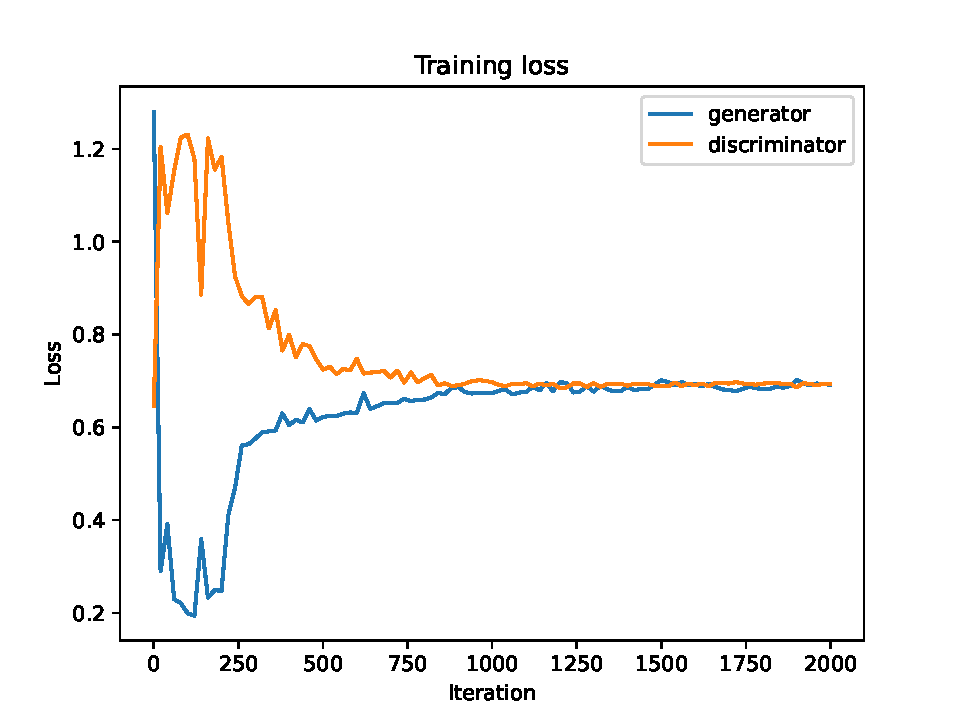
\includegraphics[width=0.95\linewidth]{figures/training_loss_1.pdf}
    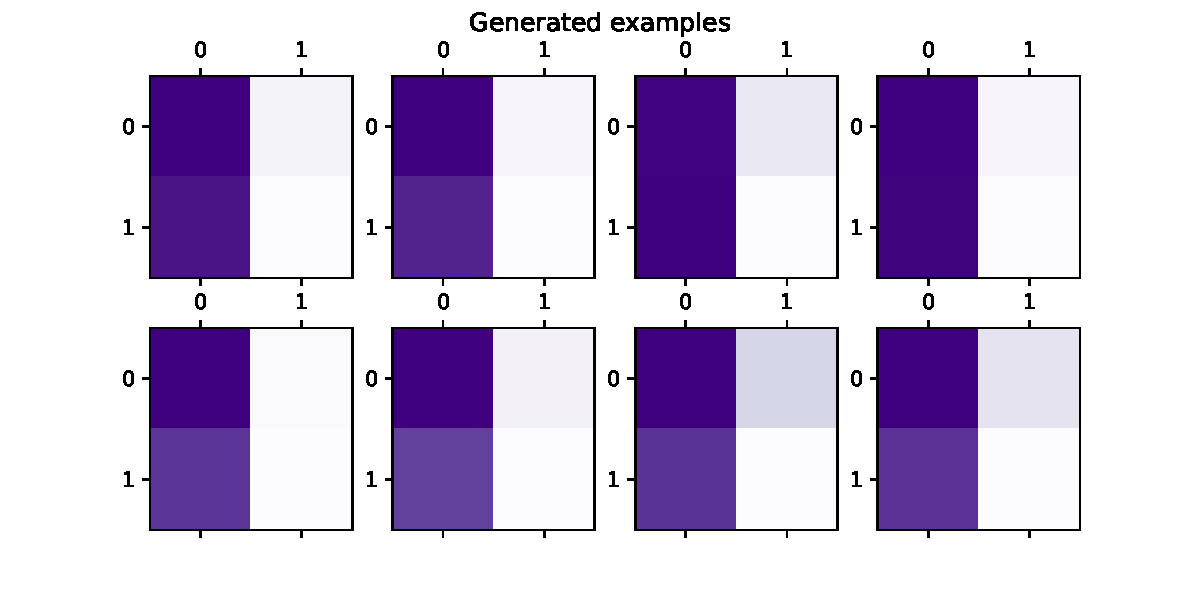
\includegraphics[width=0.95\linewidth]{figures/examples_1.pdf}

\column{0.5\textwidth}
\centering
    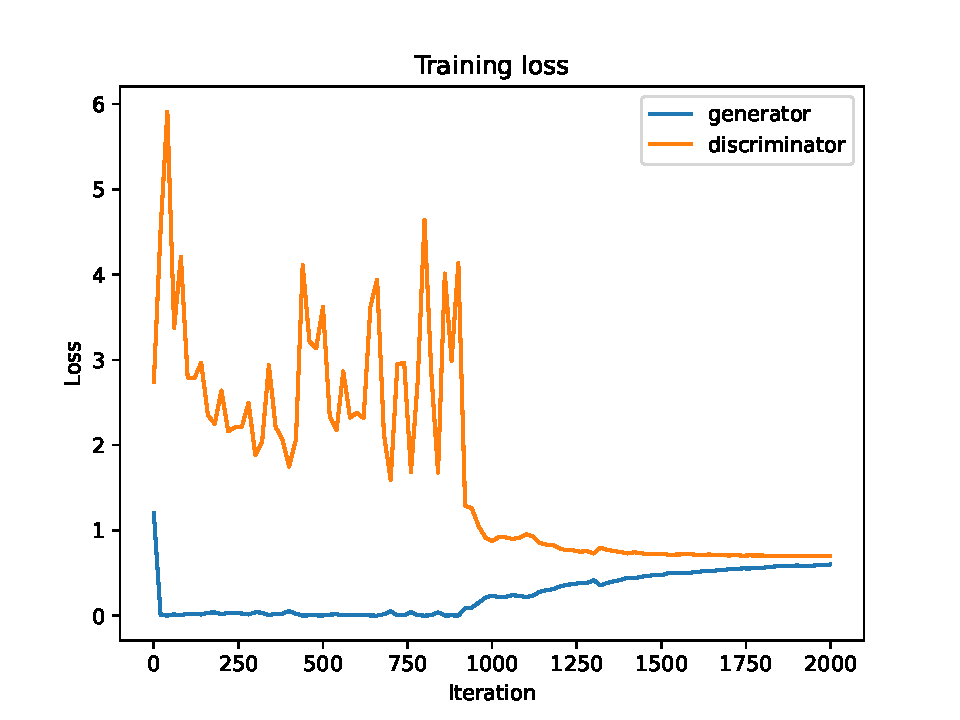
\includegraphics[width=0.95\linewidth]{figures/training_loss_2.pdf}
    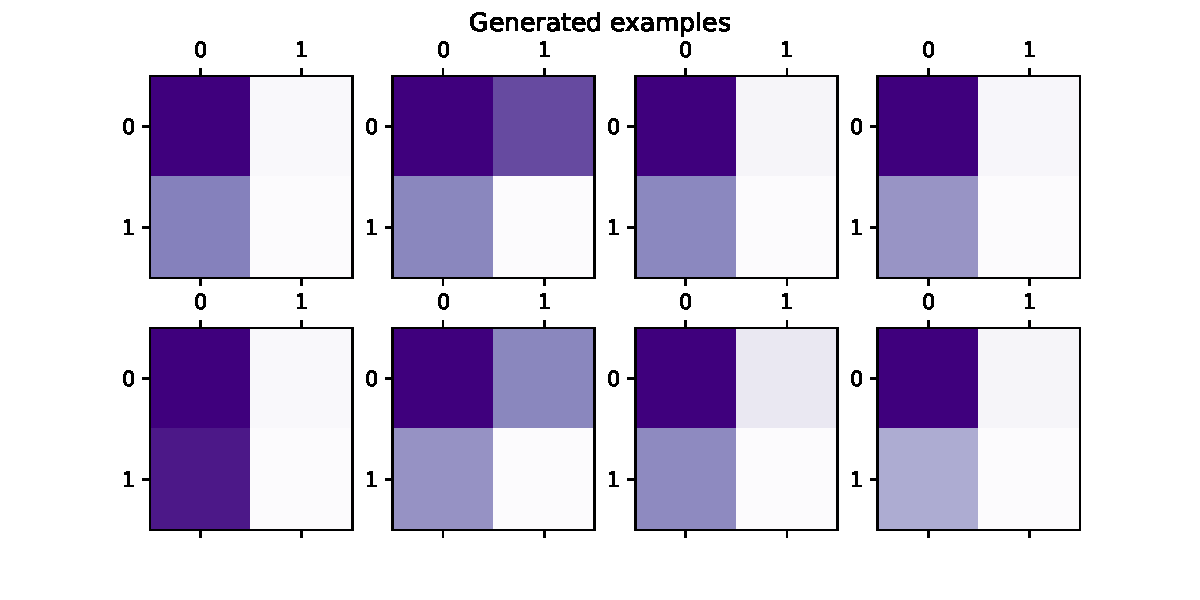
\includegraphics[width=0.95\linewidth]{figures/examples_2.pdf}
\end{columns}

\end{frame}

\begin{frame}[fragile]{Software design and implementation}
\begin{itemize}
    \item JAX throughout: just take gradients of the loss methods.
    \item Simple, but extensible API implementing completely quantum GANs (generator and discriminator):
    \begin{minted}[fontsize=\footnotesize]{python}
g = gan.BatchGAN(4, 1, 4, 1, 5,
                 entanglers=qml.CNOT, layout="random")
g.draw(...)
    \end{minted}
    \begin{center}
        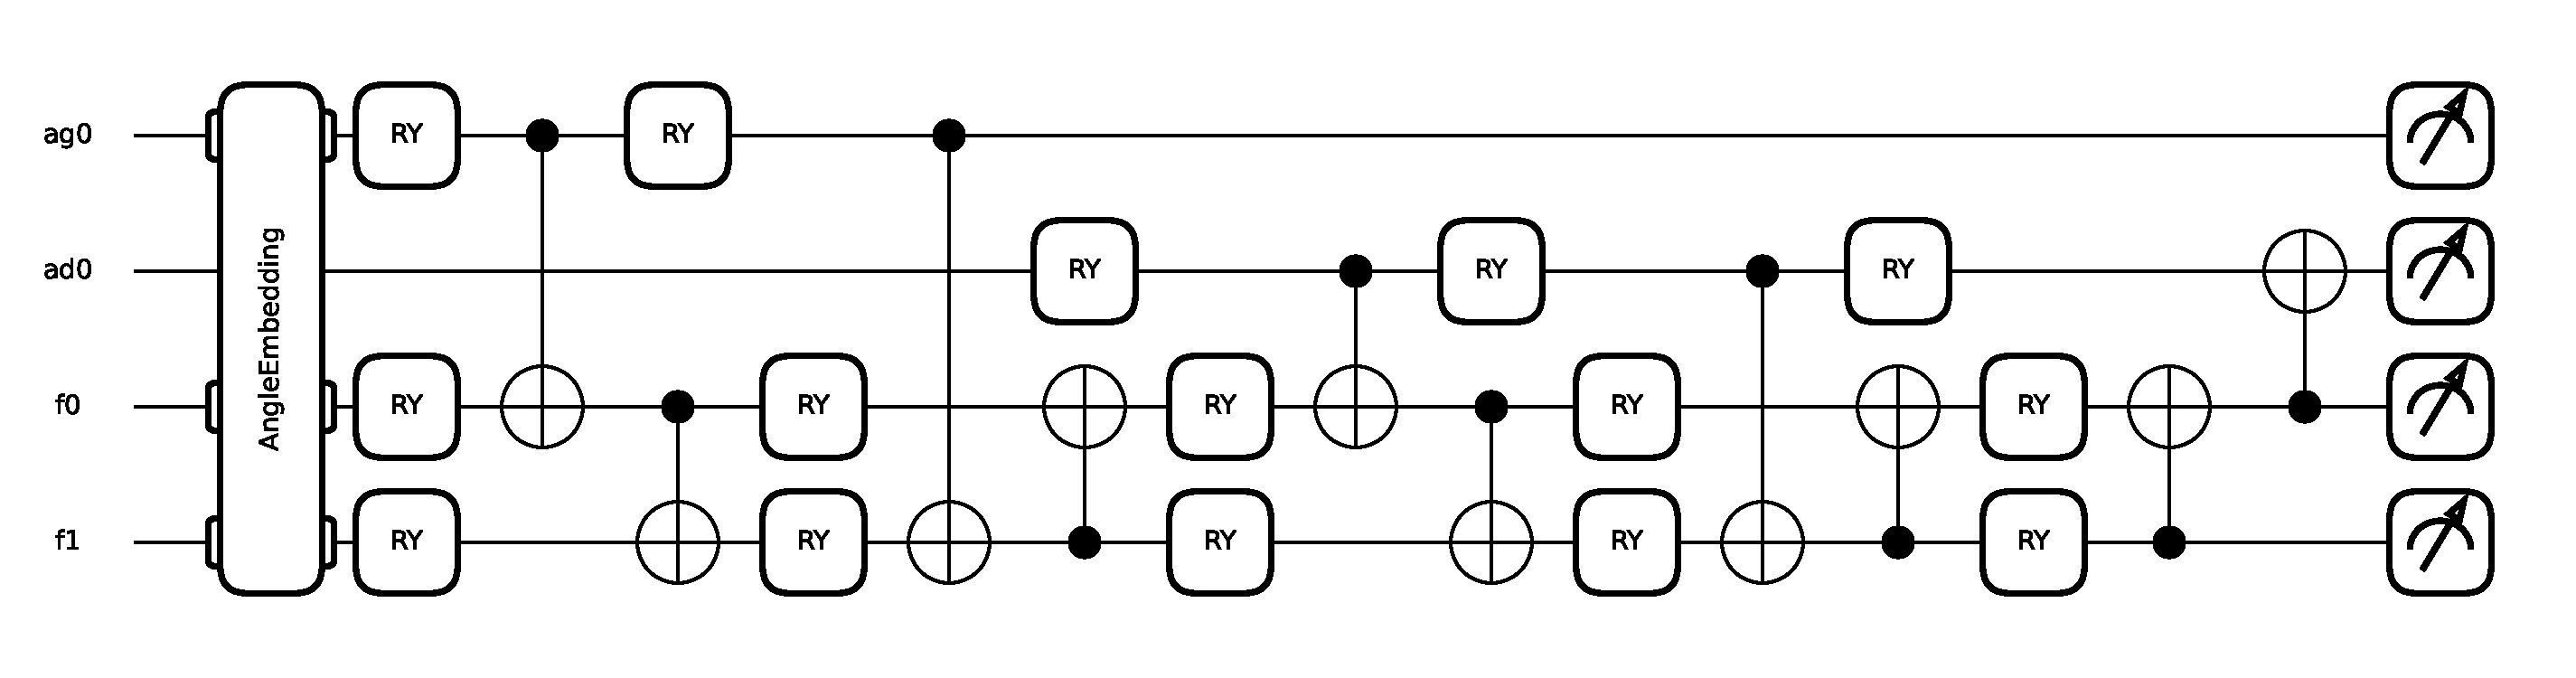
\includegraphics[width=0.9\linewidth]{figures/gates.pdf}
    \end{center}
    \item Deterministic randomness for repeatable experiments!
\end{itemize}
\end{frame}

\begin{frame}[allowframebreaks]
  \frametitle{References}
  \printbibliography
\end{frame}

\end{document}
